\subsection{End of Ninety Mile Beach}

End of Ninety Mile Beach


    Do 20.10.22    Tag 4
   


    Hukatere Campsite - Ahipara
   


   Km  70,1 - 101,1
  


  Heute lassen wir uns Zeit, wir wollen nur bis zum nächsten Campingplatz etwa 17 km entfernt laufen.
 


\begin{figure}[H]
	\centering
	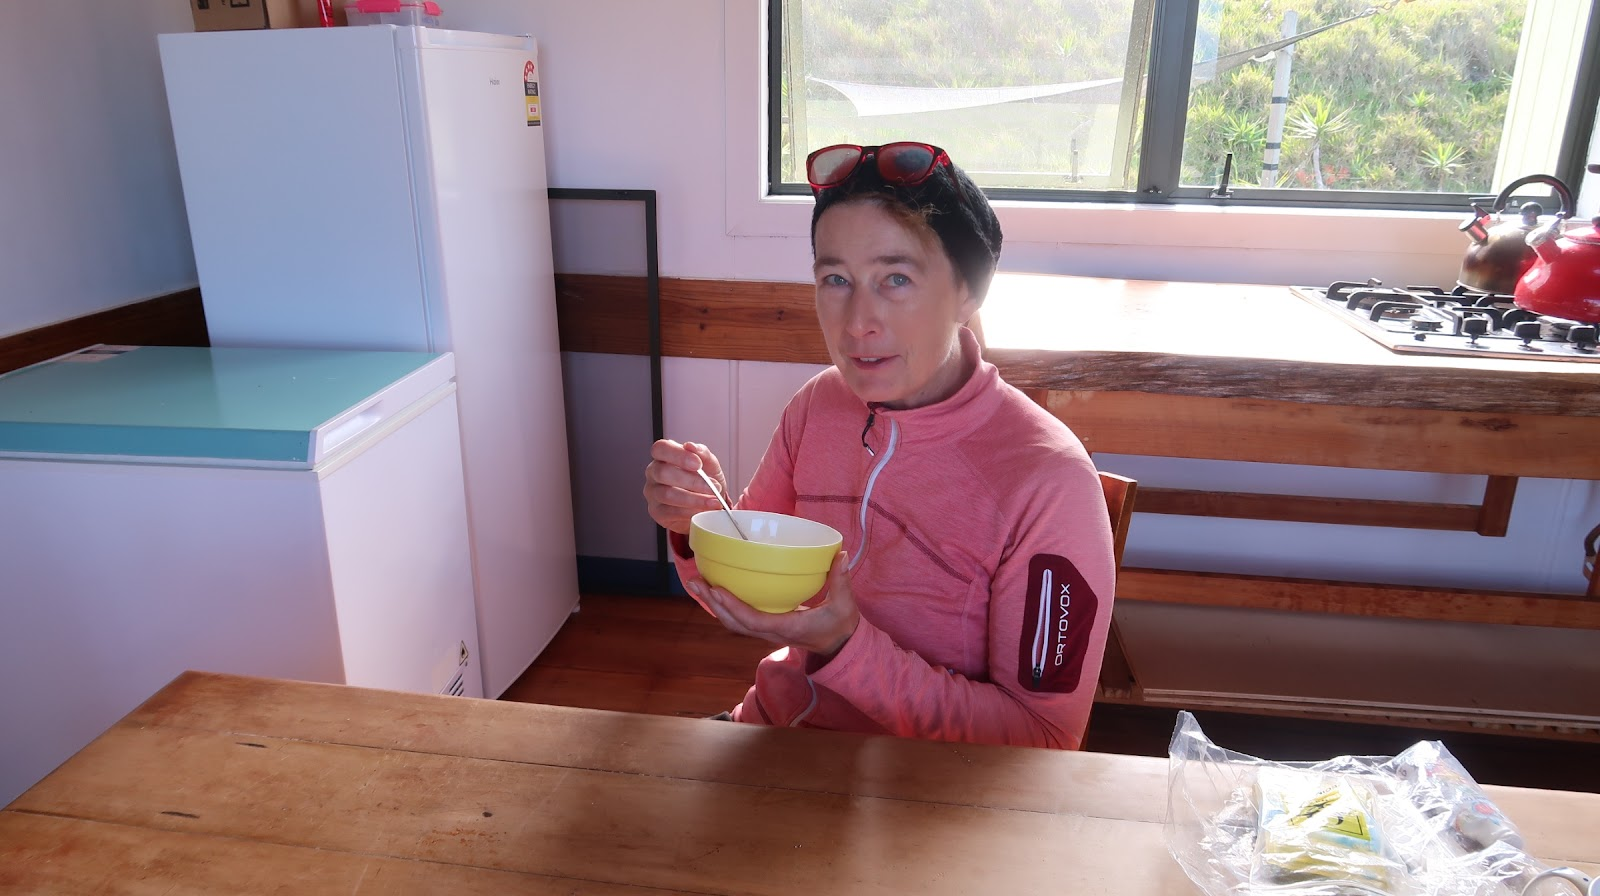
\includegraphics[width=0.5\textwidth]{end_of_ninety_mile_beach/6_1666292307198610-0.png}
	\caption{}
	\label{fig:6_1666292307198610-0}
\end{figure}

\begin{figure}[H]
	\centering
	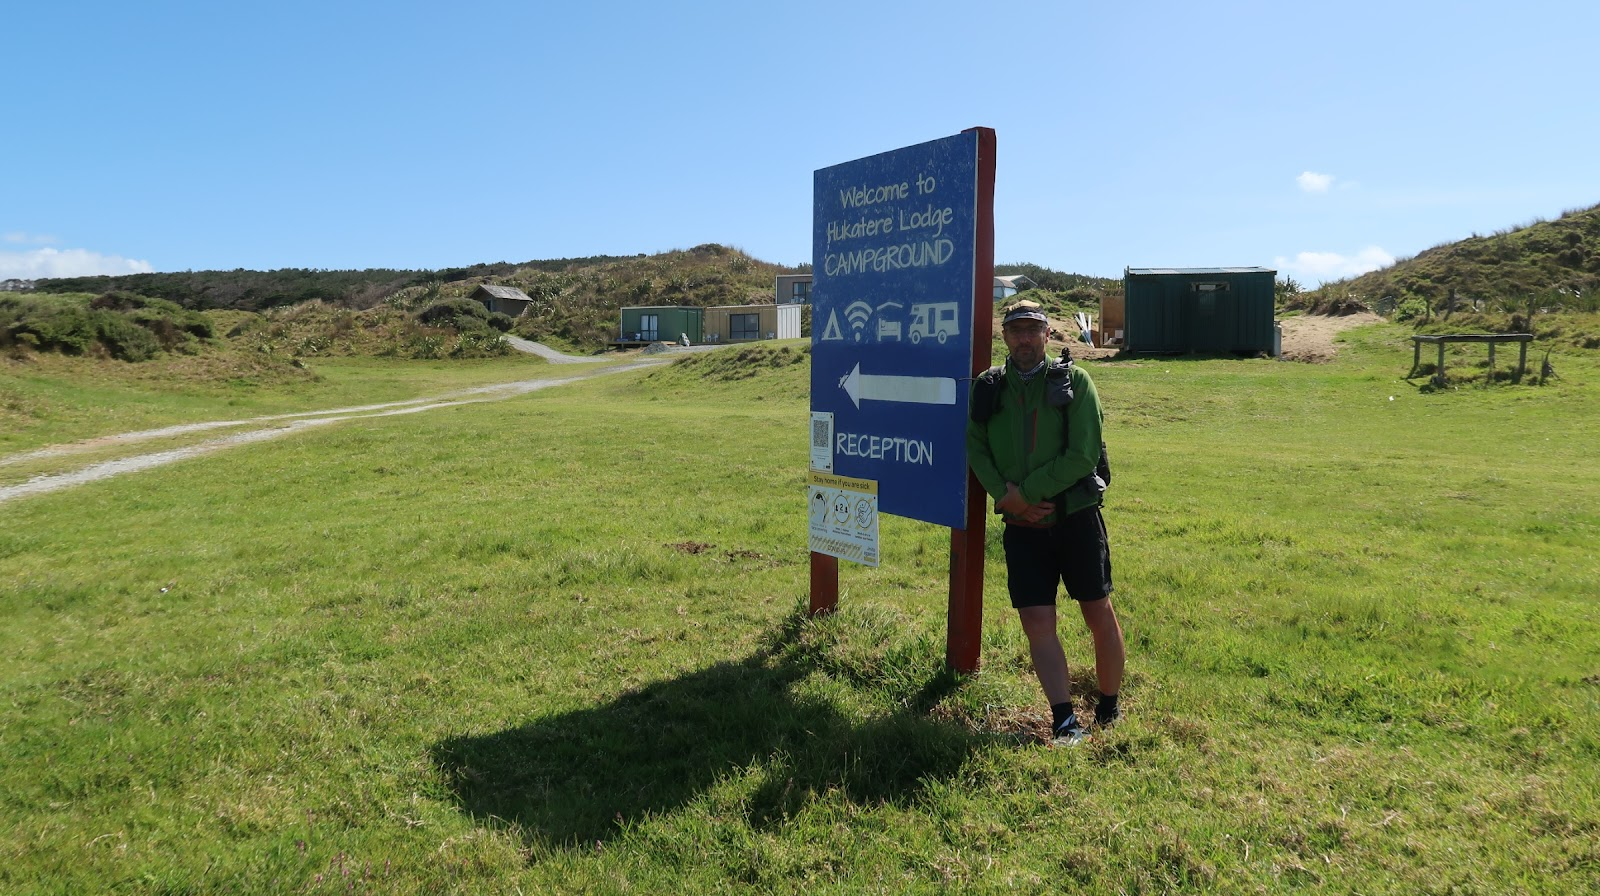
\includegraphics[width=0.5\textwidth]{end_of_ninety_mile_beach/7_1666292215000863-1.png}
	\caption{}
	\label{fig:7_1666292215000863-1}
\end{figure}

  Alle andere WanderkollegInnen sind schon länger gestartet.
 


\begin{figure}[H]
	\centering
	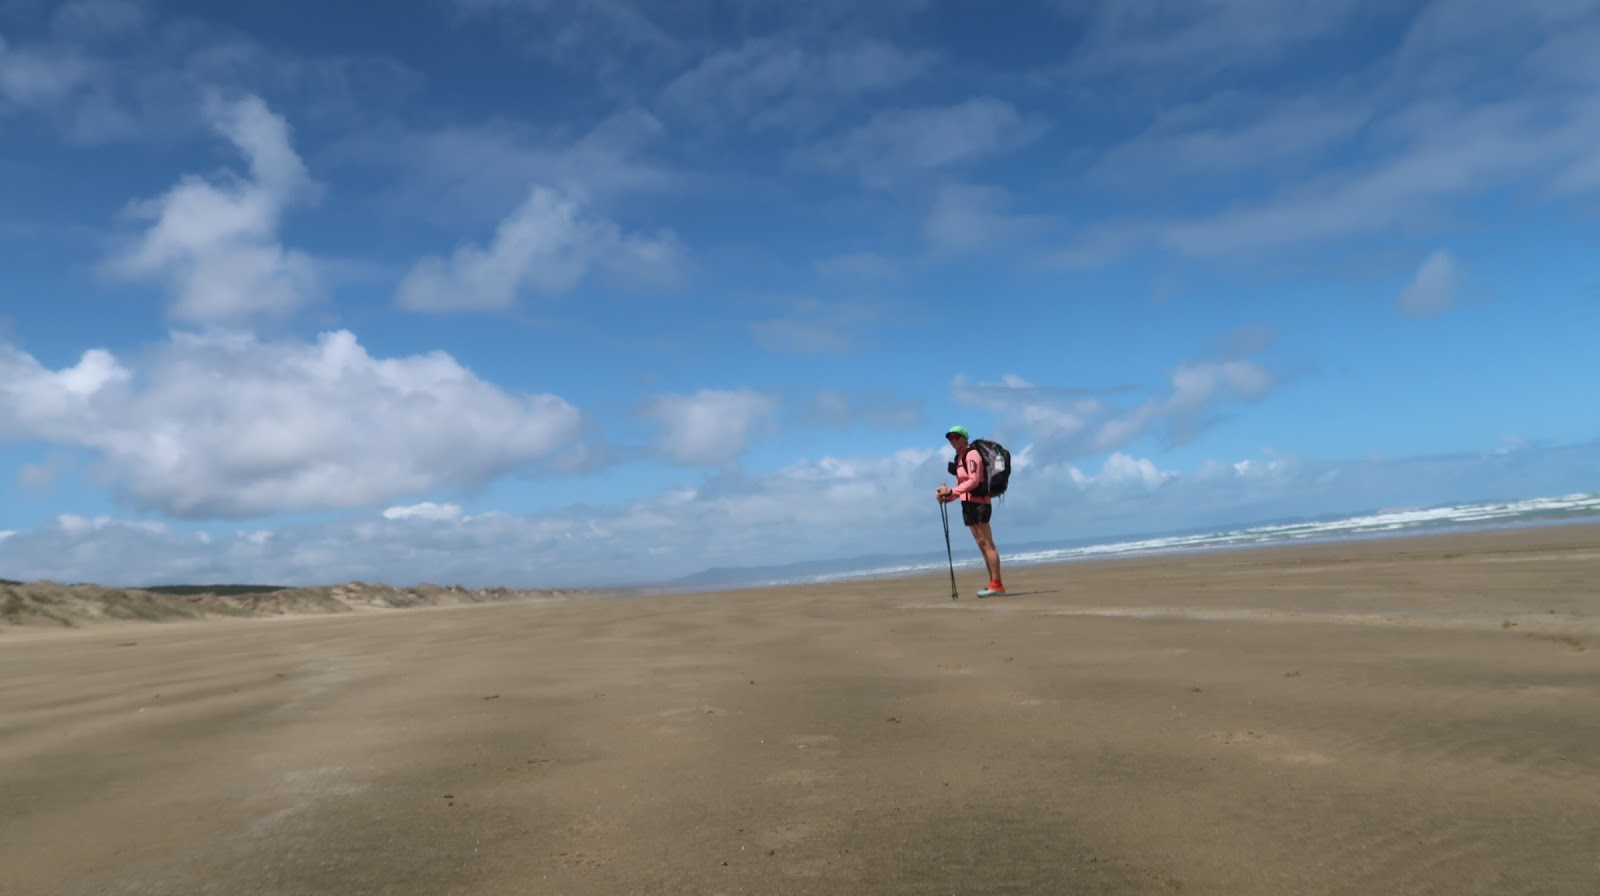
\includegraphics[width=0.5\textwidth]{end_of_ninety_mile_beach/8_1666292184476760-2.png}
	\caption{}
	\label{fig:8_1666292184476760-2}
\end{figure}

  Relativ schnell kommen wir voran und erreichen,  nach einem längeren Mittagsschläfchen, am Rand der Dünen,  kurz nach 15:00 Uhr den Abzweig zum Campingplatz. Einstimmig beschließen wir einfach weiter zu laufen, es sind ja nur noch 14  Km bis zum Ende des Strandes in Ahipara. Klingt alles ganz locker, aber hinter uns liegen zwei sehr anstrengende Tage, mit jeweils fast 30 km. Es gibt zwar keine Steigungen, aber trotzdem ist das lange  Laufen auf dem Strand nicht umbedingt förderlich für die Gelenke und Muskeln, von evtl. Blasen ganz zu schweigen.
 


  Uns geht es aber heute noch sehr gut und so erreichten wir gegen 19:00 Uhr Ahipara.
 


\begin{figure}[H]
	\centering
	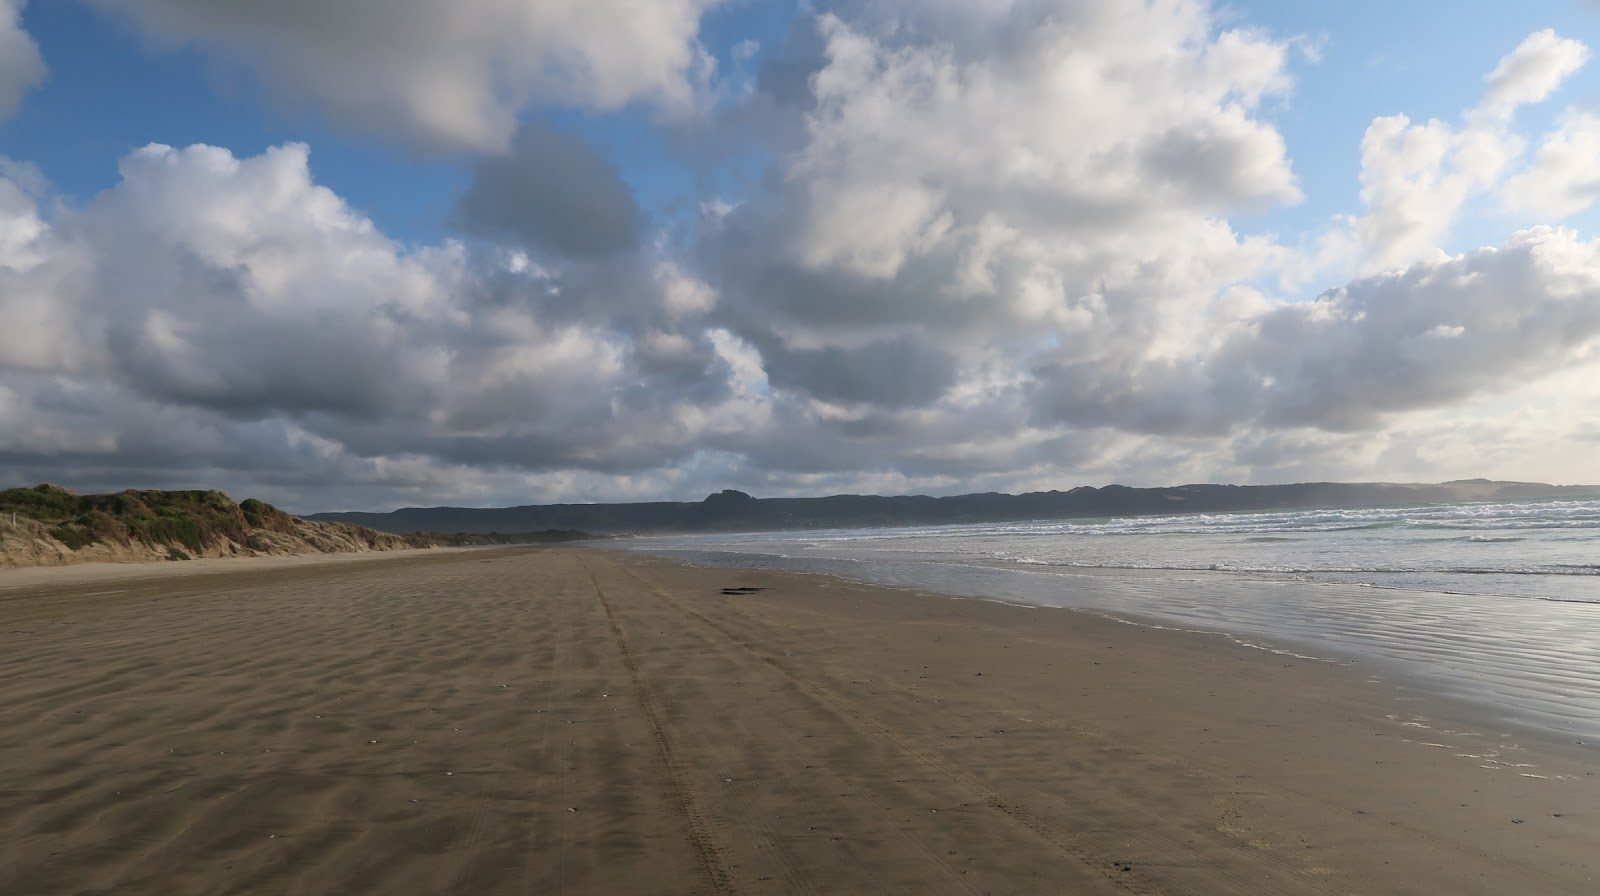
\includegraphics[width=0.5\textwidth]{end_of_ninety_mile_beach/9_1666292175623293-3.png}
	\caption{}
	\label{fig:9_1666292175623293-3}
\end{figure}

\begin{figure}[H]
	\centering
	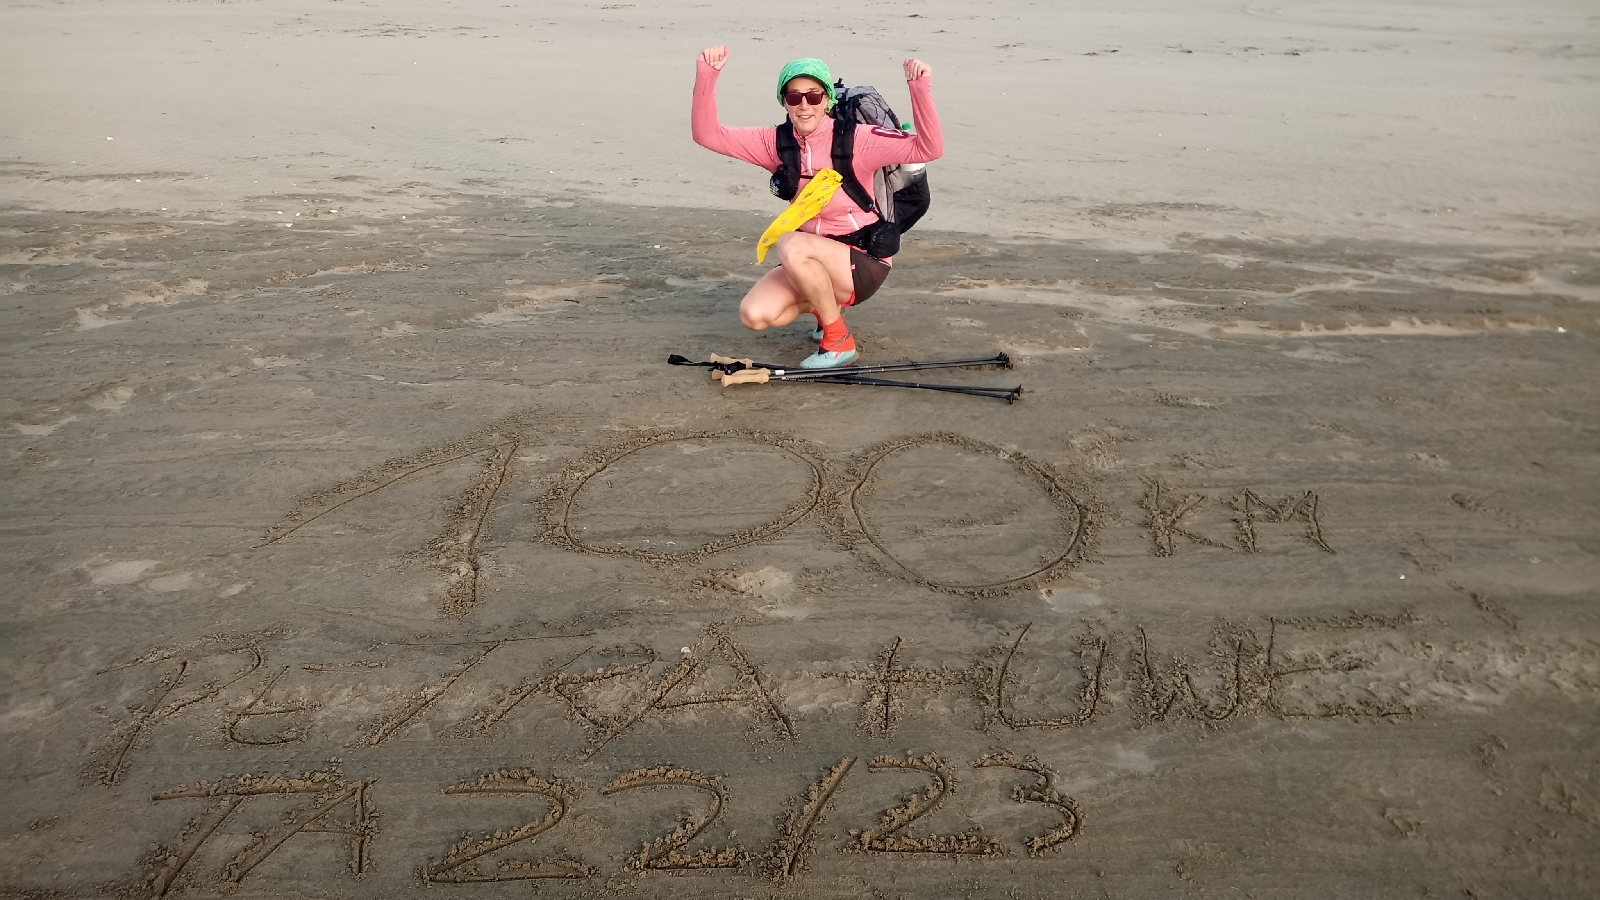
\includegraphics[width=0.5\textwidth]{end_of_ninety_mile_beach/10_1666292169096245-4.png}
	\caption{}
	\label{fig:10_1666292169096245-4}
\end{figure}

  Die ersten 100 km sind geschafft.
 


  Noch ein paar Meter bis zum wunderschönen Campingplatz, dann noch zwei Dosen Coke ein NFG ( Nudelfertiggericht) und die Nacht kann kommen.
 


\begin{figure}[H]
	\centering
	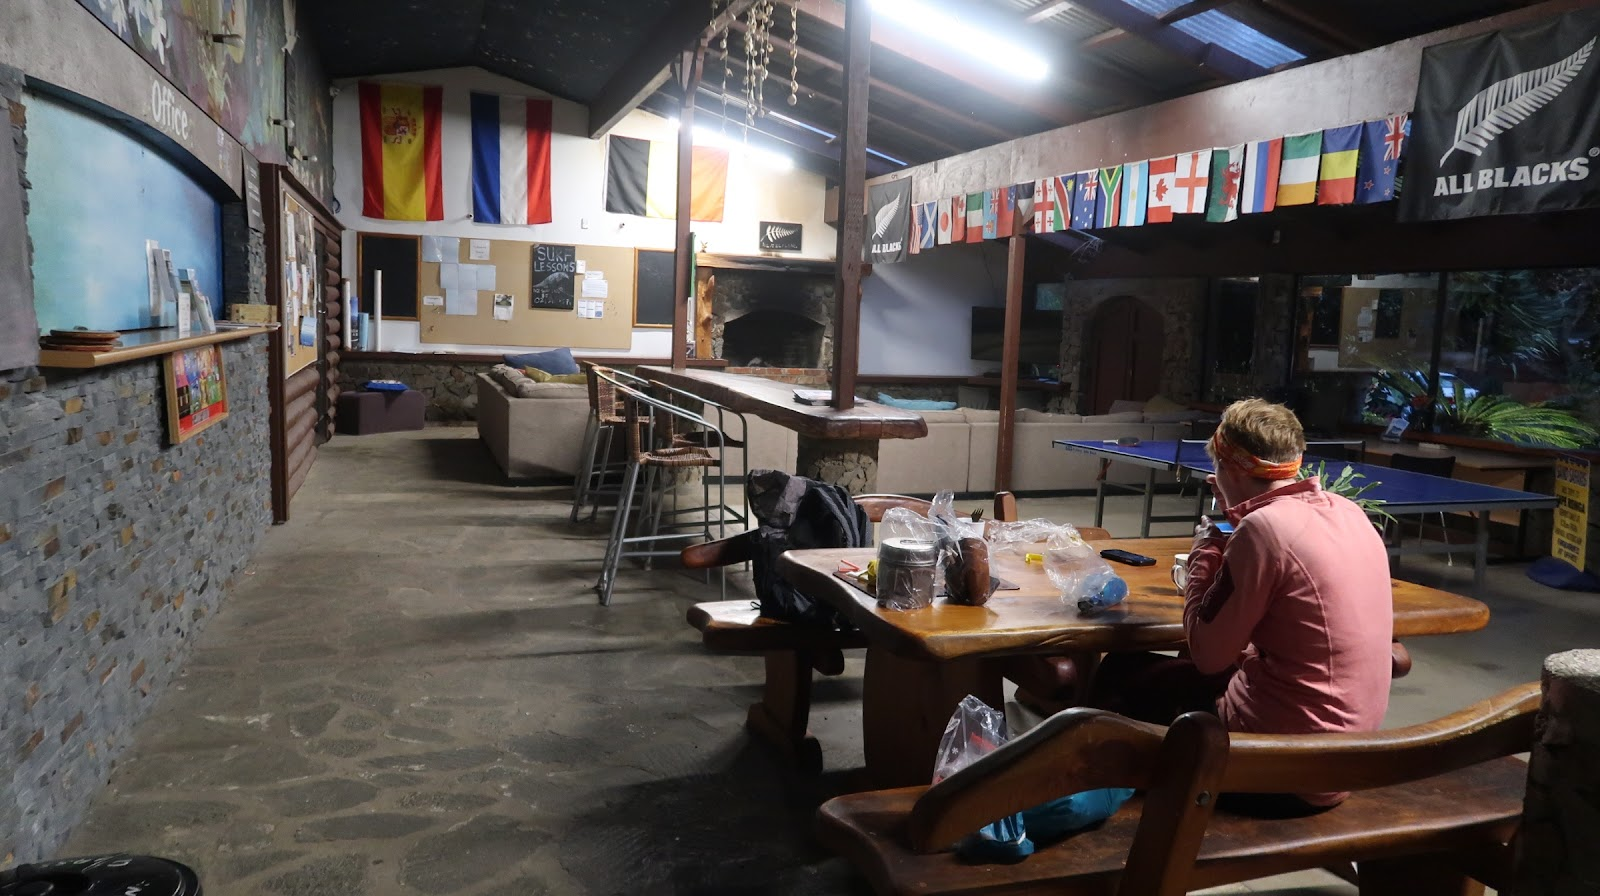
\includegraphics[width=0.5\textwidth]{end_of_ninety_mile_beach/11_1666291402036579-5.png}
	\caption{}
	\label{fig:11_1666291402036579-5}
\end{figure}

  gelaufenen 31 km
 

